%------------------------------
% Section 5 - Simulation Results
%------------------------------
\section*{5 Simulation Results}

The complete converter was simulated in LTspice XVII using transient analysis (\texttt{.tran 0 25m 0 1u startup}) with the input voltage stepped across 300\,V, 400\,V, and 500\,V. Measurements were taken during the steady-state window of 20--25\,ms. The complete schematic is shown in Figure~\ref{fig:schematic}.

\begin{figure}[H]
\centering
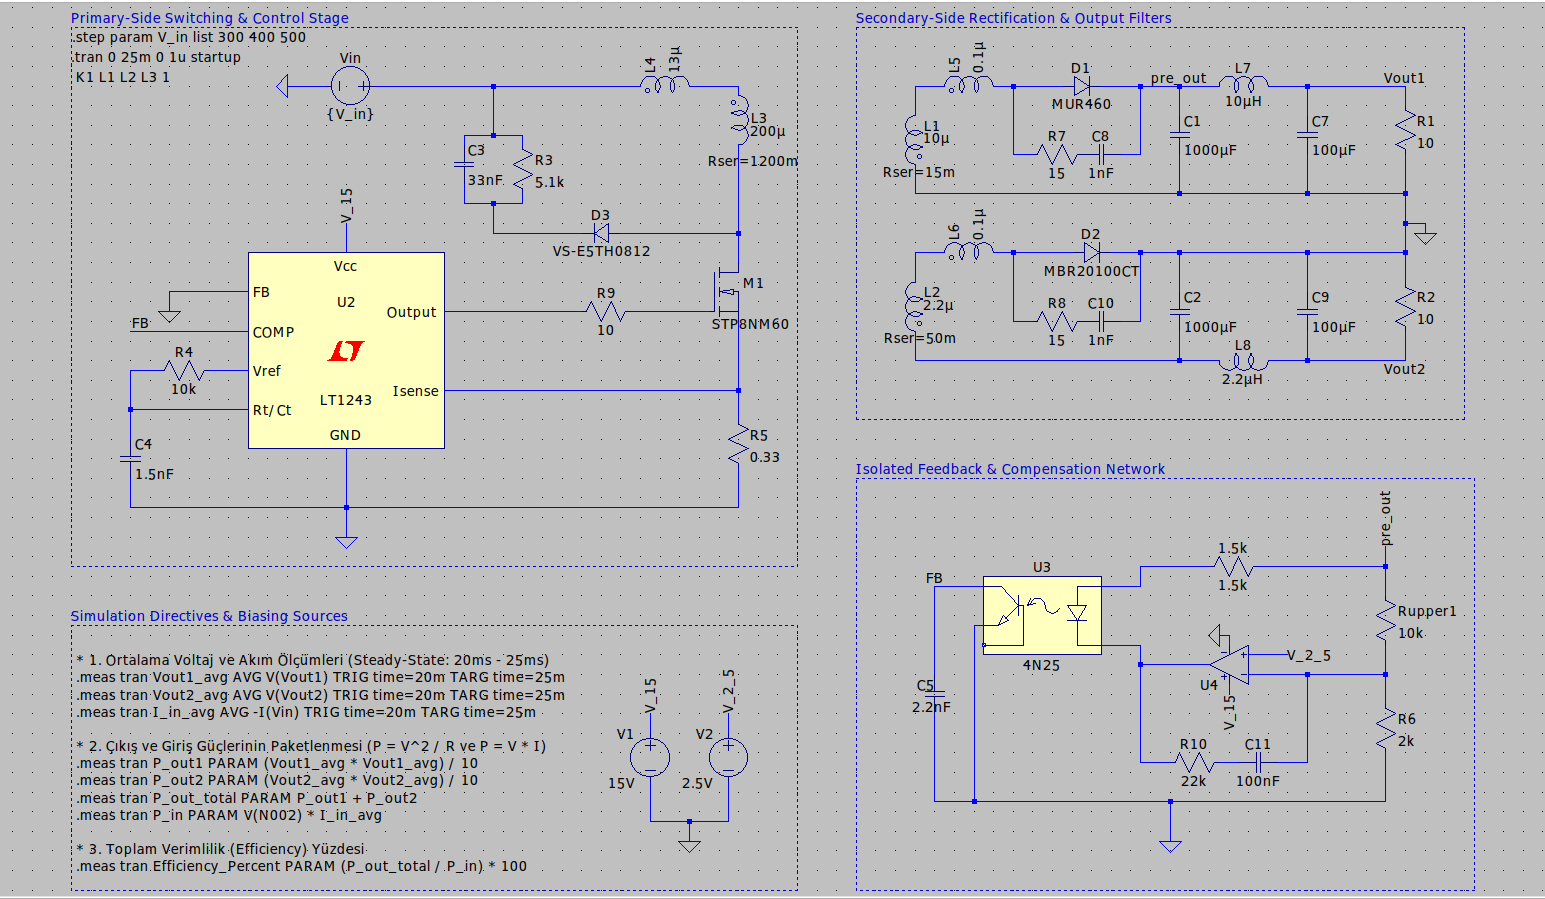
\includegraphics[width=\textwidth]{images/complete_schematic.png}
\caption{Complete LTspice Schematic}
\label{fig:schematic}
\end{figure}

\subsection*{5.1 Steady-State Output Voltages}

Table~\ref{tab:vout} summarizes the average output voltages measured over the 20--25\,ms steady-state window at each input voltage.
\begin{table}[H]
\centering
\caption{Steady-state output voltage measurements.}
\label{tab:vout}
\begin{tabular}{cccc}
\toprule
\textbf{$V_{in}$ (V)} & \textbf{$V_{out1}$ avg (V)} & \textbf{$V_{out2}$ avg (V)} & \textbf{$V_{out1}$ error} \\
\midrule
300 & 14.984 & $-6.913$ & $-0.11\%$ \\
400 & 14.984 & $-6.912$ & $-0.11\%$ \\
500 & 14.984 & $-6.912$ & $-0.11\%$ \\
\bottomrule
\end{tabular}
\end{table}

\subsection*{5.2 Power Analysis \& Efficiency}

Table~\ref{tab:power} presents the complete power analysis at each operating point.

\begin{table}[H]
\centering
\caption{Power and efficiency measurements across the input voltage range.}
\label{tab:power}
\begin{tabular}{lccc}
\toprule
\textbf{Parameter} & \textbf{$V_{in}=300$\,V} & \textbf{$V_{in}=400$\,V} & \textbf{$V_{in}=500$\,V} \\
\midrule
$P_{out,15V}$ (W) & 22.453 & 22.453 & 22.453 \\
$P_{out,-7V}$ (W) & 4.779 & 4.778 & 4.778 \\
$P_{out,total}$ (W) & 27.231 & 27.231 & 27.231 \\
$P_{in}$ (W) & 31.383 & 33.685 & 33.878 \\
$I_{in,avg}$ (A) & 0.1113 & 0.0841 & 0.0678 \\
\midrule
\textbf{Efficiency (\%)} & \textbf{86.8} & \textbf{80.8} & \textbf{80.4} \\
\bottomrule
\end{tabular}
\end{table}

All three operating points are above the 75\% minimum efficiency requirement. The best efficiency of 86.8\% is at $V_{in} = 300$\,V, where the lower voltage means less switching stress and lower snubber dissipation. Efficiency drops slightly at higher input voltages because of increased voltage stress and higher snubber losses.

\begin{figure}[H]
\centering
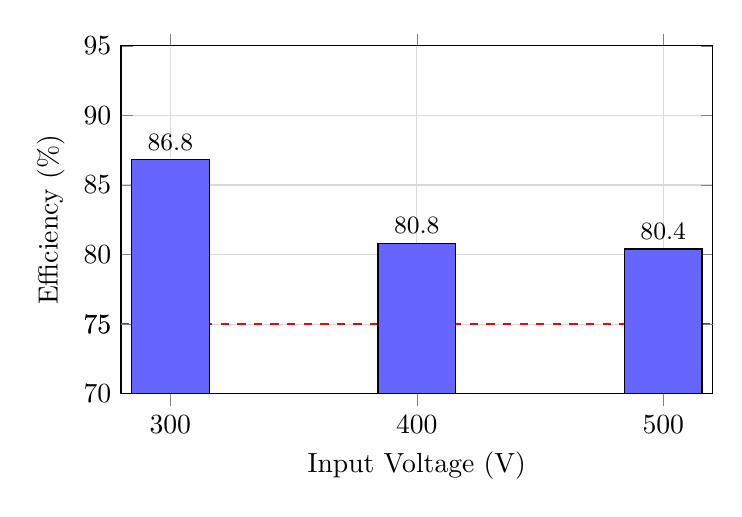
\begin{tikzpicture}
\begin{axis}[
    ybar,
    width=0.75\textwidth,
    height=6cm,
    bar width=28pt,
    ymin=70, ymax=95,
    ylabel={Efficiency (\%)},
    xlabel={Input Voltage (V)},
    symbolic x coords={300, 400, 500},
    xtick=data,
    nodes near coords,
    nodes near coords align={vertical},
    every node near coord/.append style={font=\small\bfseries},
    ytick={70,75,80,85,90,95},
    extra y ticks={75},
    extra y tick style={grid=major, grid style={red, dashed, thick}},
    grid=major,
    grid style={gray!30},
]
\addplot[fill=blue!60] coordinates {(300, 86.8) (400, 80.8) (500, 80.4)};
\end{axis}
\end{tikzpicture}
\caption{Converter efficiency as a function of input voltage. The dashed red line indicates the 75\% minimum specification.}
\label{fig:eff}
\end{figure}

\subsection*{5.3 Switching Waveforms}

The MOSFET drain-source voltage waveform shows that the RCD snubber is working correctly -- the voltage overshoot from leakage inductance stays below the 600\,V rating of the STP8NM60. The primary current has the expected sawtooth shape from current-mode control, ramping up during the on-time and resetting through the transformer during the off-time.

\begin{figure}[H]
\centering
\begin{subfigure}[t]{0.48\textwidth}
    \centering
    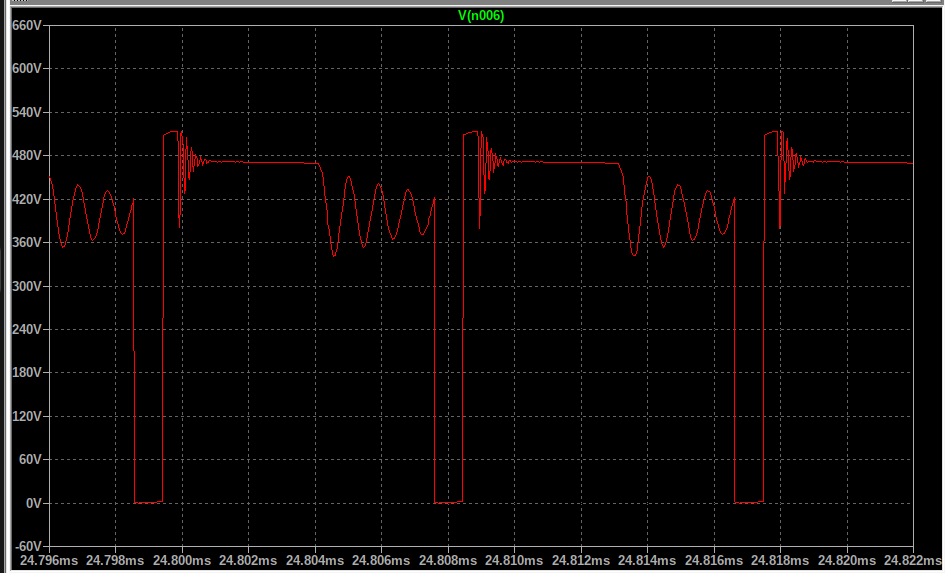
\includegraphics[width=\textwidth]{images/mosfet_vds.png}
    \caption{MOSFET Drain-Source Voltage ($V_{DS}$)}
    \label{fig:vds}
\end{subfigure}
\hfill
\begin{subfigure}[t]{0.48\textwidth}
    \centering
    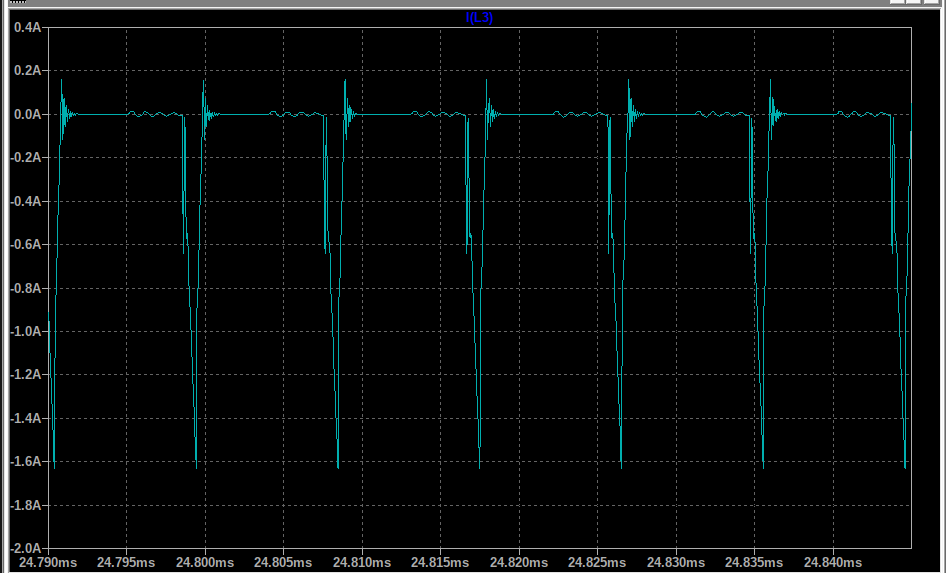
\includegraphics[width=\textwidth]{images/primary_current.png}
    \caption{Primary Current ($I_p$) at $V_{in} = 400$\,V.}
    \label{fig:ipri}
\end{subfigure}
\caption{Switching waveforms at steady state.}
\label{fig:switching}
\end{figure}

\subsection*{5.4 Startup Transient}

The \texttt{startup} directive models the LT1243's soft-start behavior. The output voltages ramp up smoothly without overshoot, reaching steady-state in about 10--15\,ms.

\begin{figure}[H]
\centering
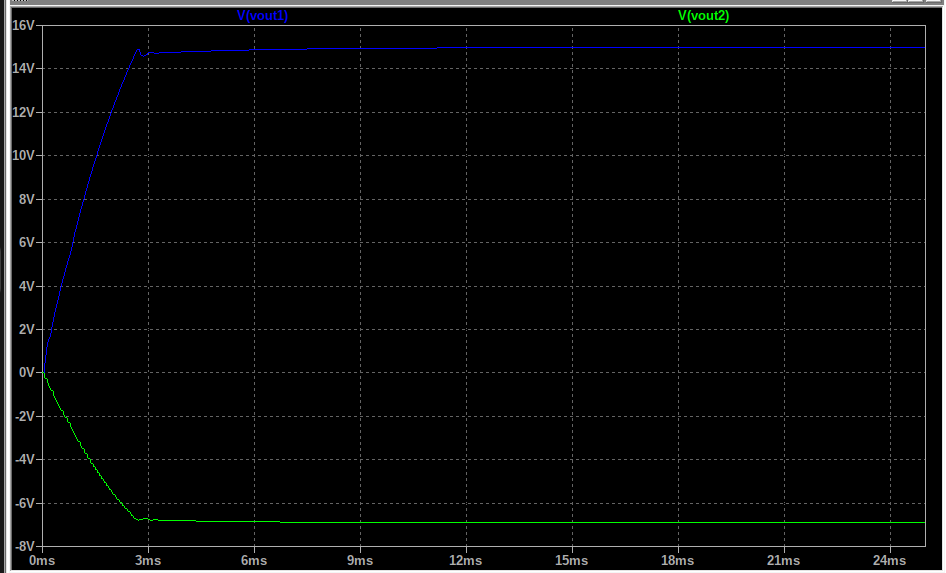
\includegraphics[width=0.9\textwidth]{images/startup_transient.png}
\caption{Output voltage startup transient (0--20\,ms).}
\label{fig:startup}
\end{figure}

\subsection*{5.5 Output Voltage Ripple}

The output ripple was measured by examining the AC component of the output voltages at steady state. Due to the combination of bulk capacitors ($1000\,\mu$F) and post-LC filters ($L_7$/$C_7$ and $L_8$/$C_9$), the ripple on both outputs is well below the 400\,mV$_{pp}$ specification.

\begin{figure}[H]
\centering
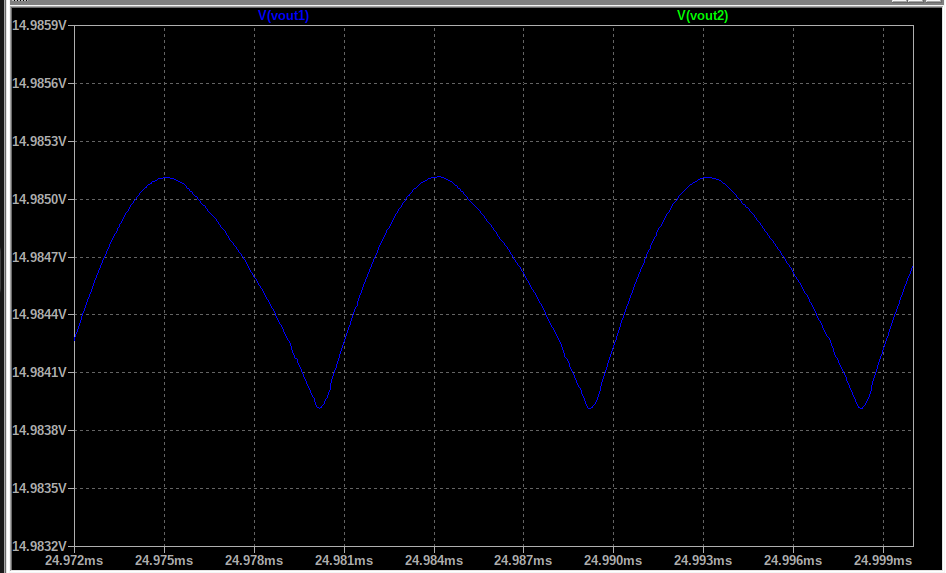
\includegraphics[width=0.9\textwidth]{images/output_ripple.png}
\caption{Output voltage ripple (AC-coupled) at $V_{in} = 400$\,V.}
\label{fig:ripple}
\end{figure}
